
\documentclass{jtetiproposalskripsi}

%-----------------------------------------------------------------
%Disini awal masukan untuk data proposal skripsi
%-----------------------------------------------------------------
\titleind{APLIKASI KESEKRETARIATAN DI BEM TEKNIK UNIVERSITAS MUHAMMADIYAH JEMBER}
\fullname{RYAN FEBRYANTO}

\idnum{1200631005}

\approvaldate{10 Januari 2015}

\degree{Sarjana Komputer}

\yearsubmit{2015}

\program{Manajemen Informatika}

\headprogram{Sarjiya, S.T., M.T., Ph.D.}

\dept{Manajemen Informatika dan Teknik Informatika}

\firstsupervisor{Sigit Basuki Wibowo, S.T., M.Eng.}
\firstnip{1976 0501 2002 12 1 002}

\secondsupervisor{Bimo Sunarfri Hantono, S.T., M.Eng.}
\secondnip{1977 0131 2002 12 1 003}


%-----------------------------------------------------------------
%Disini akhir masukan untuk data proposal skripsi
%-----------------------------------------------------------------

\begin{document}

\cover

\approvalpage

%-----------------------------------------------------------------
%Disini akhir masukan untuk muka skripsi
%-----------------------------------------------------------------

%-----------------------------------------------------------------
%Disini awal masukan Intisari
%-----------------------------------------------------------------
\begin{abstractind}
Kesekretariatan merupakan hal yang wajib ada disetiap instansi maupun organisasi karena dengan adanya kesekretariatan suatu organisasi dapat mengatur manajemen organisasinya yang meliputi surat menyurat, data daftar anggota,  data inventaris maupun data-data lainya yang berhubungan dengan manajemen organisasi tersebut. Begitu juga dengan organisasi kemahasiswaan di fakultas teknik yaitu Badan Esekutif Mahasiswa (BEM), dalam pelaksanakannya BEM fakultas teknik masih menggunakan aplikasi spreadsheet atau pencatatan manual pada Microsoft Office  untuk mengatur kesekretariatannya seperti dalam pencatatan surat masuk dan surat keluar,data daftar inventaris yang ada di kantor BEM serta pencatatan dokumen – dokumen lainya, dengan masih menggunakan pencatatan manual pada Microsoft Office  hal ini kurang efektif dan efesien serta membutuhkan waktu pengerjaan yang tidak sedikit mengingat banyak data-data ataupun surat-surat yang harus di catat maupun disimpan sebagai dokumen.

Dari permasalah tersebut munculah gagasan untuk membuat suatu aplikasi berbasis desktop dengan menggunakan bahasa pemograman java, yang dimana aplikasi tersebut dapat mengakomodir pekerjaan dan kegiatan yang menyangkut  kesekretariatan di Badan Esekutif Mahasiswa (BEM) fakultas teknik. 

Aplikasi ini diharapkan menjadi solusi untuk permasalahan dalam hal pencatatan surat-menyurat,pengumpulan data  yang efesian dan efektif serta penyediaan suatu database yang didalamnya terdapat data-data yang berkenaan kesekretariatan yang ada di BEM fakultas teknik.


\bigskip
\textbf{Kata kunci} : \emph{Kesekretariatan, Microsoft Office , Desktop, Java}.
\end{abstractind}
%-----------------------------------------------------------------
%Disini akhir masukan Intisari
%-----------------------------------------------------------------

\tableofcontents
\addcontentsline{toc}{chapter}{DAFTAR ISI}
\selectlanguage{bahasa}\clearpage\pagenumbering{arabic}\setcounter{page}{1}

%-----------------------------------------------------------------
%Disini awal masukan untuk Bab
%-----------------------------------------------------------------
\chapter{LATAR BELAKANG}

\section{Latar Belakang Masalah}
Badan Eksekutif Mahasiswa Fakultas Teknik adalah organisasi intra kampus yang berkedudukan di fakultas teknik Universitas Muhammadiyah Jember, yang anggotanya kepengurusannya terdiri dari berbagai mahasiswa jurusan yang terdapat di fakultas teknik yaitu jurusan Manajemen Informatika, Teknik Informatika,Mesin,Sipil dan Elektro,dimana dari mahasiswa dari berbagai jurusan tersebut menjadi pengurus BEM fakultas teknik selama setahun masa jabatan sebelum diganti oleh pengurus yang baru, dalam kegiatannya BEM-F membuat program kerja selama setahun yang mencakup kegiatan di dalam kampus ataupun di luar kampus.

Aplikasi  merupakan suatu program yang siap untuk digunakan yang dibuat unuk melaksanakan suatu fungsi bagi pengguna jasa aplikasi serta penggunaan aplikasi lain yang dapat digunakan oleh suatu sasaran yang akan dituju, aplikasi dapat berbasis destop ataupun berbasis mobile.

Java adalah bahasa pemograman multi platform dan multi device, dimana aplikasi yang di bangun atau dibuat dari bahasa pemograman java dapat dijalankan di berbagai operasi sistem, aplikasi berbasis java dikompulasikan kedalam p-code dan bisa dijalankan dengan Java Virtual Machine.

Dalam pengolahan data-data kesekretariatan BEM Fakultas Teknik masih menggunakan aplikasi pencatatan manual pada Microsoft Office dan pengolahan data untuk melakukan pencatatan manual dengan mengumpulkan surat masuk dan surat keluar serta pendataan kegiatan yang akan dilaksanakan.  Kendala muncul dengan menggunakan pencatatan manual yaitu masalah keakuratan data dan keamanan data, dengan adanya pergantian pengurus setiap tahunnya sering menimbulkan masalah hilangnya data-data dari pengurus sebelumnya ke pengurus baru, kebanyakan data-data tersebut hilang karena kurangnya manajemen data ataupun pencatatan yang masih manual.

Berdasarkan latar belakang di atas, penulias merancang dan membuat aplikasi kesekretariatan di BEM fakultas teknik, dengan dibuatnya aplikasi tersebut diharapkan dapat mengatasi masalah-masalah yang muncul berkaitan dengan pencatatan,pengumpulan dan pengaturan manejemen yang terkomputerisasi.

\section{Perumusan Masalah}
Berdasarkan latar belakang diatas maka identifikasi masalah yang muncul dalam penelitian ini adalah:	 
\begin{itemize}
\item[A.] Bagaimana cara mengubah memanajemen kesekretariatan BEM Fakultas Teknik dari manual menjadi komputerisasi.
\item[B.] Bagaimana membuat aplikasi kesekreariatan pada BEM Fakultas Teknik menggunakan Java.
\end{itemize}

\section{Batasan Masalah}

Agar penelitian yang dilakukan lebih terarah sesuai tujuan penelitian serta memudahkan dalam pengumpulan dan pengolahan data,analisa serta menarik kesimpulan, maka ruang lingkup penelitian dibatasi dan di asumsikan sebagai berikut : 
\begin{itemize}
\item[A.] Pembangunan aplikasi yang mencakup pendataan surat masuk dan surat keluar, data inventory, dan data anggota.
\item[B.] Laporan kegiatan program kerja yang sudah terlaksana dan laporan pertangungjawaban kegiatan.
\item[C.] Menggunakan bahasa pemograman Java.
\end{itemize}

\section{Tujuan Penelitian}
Adapun tujuan dari tugas akhir ini adalah merancang aplikasi kesekretariatan pada BEM Fakultas Teknik sebagai berikut :
\begin{itemize}
\item[A.] Membuat system pengelolaan memanajemen kesekretariatan yang terintegrasi dengan system komputerisasi.
\item[B.] Membantu BEM Fakultas Teknik untuk lebih efesien dan efektif dalam mengelola kesekretariatannya
\end{itemize}


\section{Manfaat Penelitian}
Adapun yang menjadi manfaat dari penelitian yang akan dilakukan adalah :
\begin{itemize}
\item[A.] Dapat meminimalisir kesalahan, perbedaan data dan kehilangan data-data.
\item[B.] Mempermudah dalam pencatatan biodata anggota pengurus yang aktif maupun yang sudah tidak aktif.
\end{itemize}

%-------------------------------------------------------------------------------
\chapter{TINJAUAN PUSTAKA DAN DASAR TEORI}               
\section{Landasan Teori}
\subsection{Sistem Informasi Manajemen }
Sistem Informasi Manajemen adalah sistem perensanaan bagian bagian dari pengendalian internal suatu bisnis yang meliputi pemanfaatan manusia, dokumen, teknologi, dan prosedur oleh akuntansi manajemen untuk memecahkan masalah bisnis. Sistem informasi manajemen dibedakan dengan sistem informasi biasa karena SIM digunakan untuk menganalisis sistem informasi lain yang diterapkan pada aktivitas operasional organisasi. Secara akademis, istilah ini umumnya digunakan untuk merujuk pada kelompok metode manajemen informasi yang bertalian dengan otomasi atau dukungan terhadap pengambilan keputusan manusia, misalnya sistem pendukung keputusan, sistem pakar, dan sistem informasi eksekutif. Sistem Informasi Manajemen merupakan sistem yang menghasilkan hasil keluaran (output) dengan menggunakan masukan (input) dan berbagai proses yang diperlukan untuk memenuhi tujuan tertentu dalam suatu kegiatan manajemen.

Menurut Kertahadi (1995) : Sistem Informasi Manajemen (SIM) dapat didefinisikan sebagai suatu alat untuk menyajikan informasi dengan cara sedemikian rupa sehingga bermanfaat bagi penerimanya...
	
Menurut Murdick dan Ross  (1993) : Tujuan sistem informasi manajemen adalah untuk menyajikan informasi guna pengambilan keputusan pada perencanaan, pemrakarsaan, pengorganisasian, pengendalian kegiatan operasi subsistem suatu perusahaan dan menyajikan sinergi organisasi pada proses.

\subsection{Sistem}
Menurut Jogiyanto (2005: 2) dalam buku yang berjudul Analisis dan Desain Sistem Informasi menjelaskan bahwa: “sistem adalah kumpulan dari elemen-elemen yang berinteraksi untuk mencapai suatu tujuan-tujuan tertentu”.

Menurut Scott (1996) : mengatakan sistem terdiri dari unsur-unsur seperti masukan (input), pengolahan (processing), serta keluaran (output). Ciri pokok sistem menurut Gapspert ada empat, yaitu sistem itu beroperasi dalam suatu lingkungan, terdiri atas unsur-unsur, ditandai dengan saling berhubungan dan mempunyai satu fungsi atau tujuan utama.

Menurut Mc. Leod (1995) : sistem sebagai sekelompok elemen-elemen yangterintegrasi dengan maksud yang sama untuk mencapai suatu tujuan. Sumberdaya mengalir dari elemen output dan untuk menjamin prosesnya berjalan dengan baik maka dihubungkan mekanisme control...

Menurut Suradinata (dalam Schronderberg, 1996) : sistem adalah Komponen-komponen sistem saling berhubungan satu sama lainnya. Suatu keseluruhan tanpa memisahkan komponen pembentukannya. Bersama-sama dalam mencapai tujuan. Memiliki input dan output yang dibutuhkan oleh sistem lainnya. Terdapat proses yang merubah input menjadi output. Menunjukan adanya entropi terdapat aturan Terdapat subsistem yang lebih kecil, terdapat deferensiasi antar subsistem. Terdapat tujuan yang sama meskipun mulainya berbeda.


\subsection{Sistem Informasi}
Sistem Informasi adalah kombinasi dari teknologi informasi dan aktivitas orang yang menggunakan teknologi itu untuk mendukung operasi dan manajemen dalam arti yang sangat luas, istilah sistem informasi yang sering digunakan merujuk kepada interaksi antara orang, proses, algoritmik, data, dan teknologi.

Menurut Jogiyanto (2005: 196) dalam  bukunya yang berjudul Analisis dan Desain Sistem Informasi  menyebutkan  bahwa:  “desain  sistem  dapat  didefinisikan  sebagai penggambaran, perencanaan, dan pembuatan sketsa atau pengaturan dari beberapa elemen yang terpisah dari satu kesatuan yang utuh dan berfungsi”.

Menurut Stair (1992) : menjelaskan bahwa sistem informasi berbasis komputer (CBIS) dalam suatu organisasi terdiri dari komponen-komponen berikut :
\begin{itemize}
\item Hardware, yaitu perangkat keras komponen untuk melengkapi kegiatan memasukan data, memproses data dan keluaran data.
\item Software, yaitu program dan instruksi yang diberikan kekomputer.
\item Database, yaitu kumpulan data dan informasi yang diorganisasikan sedemikian rupa sehingga mudah diakses pengguna sistem informasi.
\item Telekomunikasi, yaitu komunikasi yang menghubungkan antara pengguna sistem dengan sistem komputer secara bersama-sama kedalam suatu jaringan kerja yang efektif.
\item Manusia, yaitu personil dari sistem informasi, meliputi manajer, analis, programmer, operator dan bertanggung jawab terhadap perawatan sistem.
\item Prosedur, yakni tata cara yang meliputi strategi, kebijakan, metode dan peraturan-peraturan dalam menggunakan sistem informasi berbasis komputer.
\end{itemize}

Menurut Jogiyanto (2005: 11) dalam buku yang berjudul Analisis dan Desain Sistem Informasi, menyebutkan bahwa: Sistem informasi  adalah suatu sistem di dalam suatu organisasi yang mempertemukan kebutuhan pengolahan transaksi harian, mendukung operasi, bersifat manajerial dan kegiatan strategi dari suatu organisasi dan menyediakan pihak luar tertentu dengan laporan-laporan yang diperlukan.

Menurut Ladjamudin (2005: 13) dalam buku yang berjudul Analisis dan Desain Sistem Informasi mendefinisikan bahwa: ”sisutem informasi adalah sekumpulan prosedur organisasi yang pada saat dilaksanakan akan memberikan informasi bagi pengambil keputusan  dan  atau untuk mengendalikan organisasi”.

Menurut Yafie (2011: 194) sistem pengolahan informasi memiliki sistem fungsional seperti sistem perangkat keras, sistem pengoperasian (operating system), sistem komunikasi, dan sistem database. Ia juga memiliki subsistem seperti masukan pesanan dan penagihan, dan daftar gaji serta personalia...

\subsection{Perancangan Sistem}
Perancangan sistem adalah merancang atau mendesain suatu sistem yang baik, yang isinya adalah langkah-langkah operasi dalam proses pengolahan data dan prosedur untuk mendukung operasi sistem. 
Menurut Santoso (2011: 19) : Proses-proses standard yang digunakan untuk membangun suatu sistem informasi meliputi langkah-langkah berikut ini: 
\begin{itemize}
\item Analisa 
\item Desain 
\item Implementasi 
\item Maintenance 
\end{itemize}
Pada perkembangannya, proses-propses standar tadi dituangkan dalam satu metode yang dikenal dengan nama Systems Development Life Cycle (SDLC) yang merupakan metodologi umum dalam pengembangan sistem  yang menandai kemajuan dari usaha analisa dan desain.

Menurut Santoso (2011: 18) : Analisa sistem didefinisikan sebagai bagaimana memahami dan menspesifikasi dengan detail apa yang harus dilakukan oleh sistem. Sedangkan sistem desain diartikan sebagai menjelaskan dengan detail bagaimana bagian-bagian dari sistem informasi di implementasikan. Analisa dan desain sistem informasi (ANSI) bisa didefinisikan sebagai: Proses organisasional kompleks dimana sistem informasi berbasis komputer di implementasikan.

%-------------------------------------------------------------------------------
\chapter{METODOLOGI}

\section{Alat dan Bahan}
Bahan yang digunakan dalam penelitian ini adalah:

\vspace{-0.5cm}

\begin{enumerate}[a.]
\begin{singlespace}
\itemsep0em
\item Laptop/PC (1 unit),
\item Sistem Operasi (Windows 7),
\item Neatbean IDE 7.1.2 (Java),
\item Powerdesigner (DFD Diagram)
\item XAMPP(Mysql database),
\item Ireport(Desainer Laporan).
\end{singlespace}
\end{enumerate}

\section{Teknik Pengumpulan Data}

Metode atau teknik pengumpulan data yang digunakan dalam penelitian ini adalah dengan menggunakan kuesioner, observasi, dan studi pustaka untuk mendapatkan data primer.
Dimana pengumpulan data utama dilakukan dengan observasi langsung kepada objek penelitian dimana dalah hal ini adalah BEMS Fakultas Teknik Universitas Muhammadiyah  Jember.
\subsection{Kuesioner}

Mencari pendapat seberapa perlunya \emph{sistem informasi} ini untuk digunakan, dengan melakukan penyebaran kuesioner untuk mengukur persepsi responden digunakan Skala Likert (Rangkuti, 1997). Pertanyaan dalam kuesioner dibuat dengan menggunakan skala 1-10 untuk mewakili pendapat dari responden. Nilai untuk skala tersebut adalah:
\begin{itemize}
\item[a.] Sangat Setuju 		: 9
\item[b.] Setuju 				: 7
\item[c.] Netral				: 8
\item[d.] Tidak Setuju			: 3
\item[e.] Sangat Tidak Setuju	: 1
\end{itemize}
Hipotesis:\\
Berdasarkan  kerangka pemikiran diatas hipotesis yang diajukan dalam penelitian ini adalah:
\begin{itemize}
\item[1.] Diduga ada pengaruh kurangnya \emph{informasi} khususnya sistem informasi yang lebih efektif dan efesien untuk pengolahan keseretariatan BEMS berpengaruh terhadap lemahnya kinerja dan manajemen informasi.
\item[2.] Diduga ada pengaruh \emph{sistem informasi} yang kurang teratur khususnya dalam manaajemen dan pengaturan keseretariatan yang mencakup data anggota,investaris BEMS berpengaruh besar terhadap kinerja anggota BEMS.
\end{itemize}
\subsection{Observasi}
Penulis melakukan observasi yaitu dengan melihat langsung pada kegiatan yang di lakukan seluruh anggota BEMS dalam melakukan agenda yang telah ditentukan sebagai kegiatan tahunan, selain itu dalam Observasi penulis melihat data-data apa saja yang biasa di catat dalam kegiatan BEMS Fakultas Teknik.
\subsection{Studi Pustaka} 
Dalam penulisan ini tidak terlepas dari data-data yang terdapat dari buku-buku yang menjadi referensi seperti pedoman penulisan skripsi, diktat dan buku-buku lain yang dapat berhubungan dengan penyusunan perancangan aplikasi kesekretaritan BEMS Teknik Universitas Muhammadiyah Jember sehingga keluaran yaitu berupa aplikasi dalam sesuai dengan harapan dan selain itu dalam studi pustaka ini sebagai landasan teori untuk menyelesaikan masalah yang dihadapi.

\section{Langkah Kerja}
Pada bagian ini memuat tahapan prosedur pengembangan yang akan digunakan. Tahapan-tahapan yang akan dilakukan dalam melakukan pengembangan, tergantung pada referensi yang digunakan. Namun secara garis besar, pada tahapan ini dibagi ke dalam 3 tahapan, yaitu:  
\\ Tahap I: Studi Pendahuluan
\\ Tahap II: Tahap Pengembangan Model
\\ Tahap III: Tahap Evaluasi/Pengujian Model
\subsection{Tahap I : Studi Pendahuluan}
\begin{itemize}
\item[a.] Tahap studi pendahuluan dilakukan dengan menerapkan pendekatan deskriptif kualitatif. Studi kualitatif diawali dengan studi literatur, kemudian studi lapangan tentang perancangan aplikasi kesekretariatan BEMS guna mendukung kinerja maupun manajemen BEMS yang efektif dan efesien.
\item[b.] Pada studi pendahuluan ini diakhiri dengan \emph{deskripsi dan analisis temuan (Model Faktual).}
\end{itemize}
\subsection{Tahap II : Tahap Pengembangan Sistem}
Dalam tahap ini  hendaknya memuat butir-butir seperti berikut:\\
\textbf{Model pengembangan:}\\
Model pengembangan dapat berupa model prosedural, model konseptual, dan model teoretik. Model prosedural adalah model yang bersifat deskriptif, yaitu menggariskan langkah – langkah yang harus diikuti untuk menghasilkan sistem yang baik. Model konseptual adalah model yang bersifat analitis yang memberikan komponen – komponen sistem yang akan dikembangkan serta keterkaitan antar komponen. Model teoretik adalah model yang menunjukkan hubungan perubahan antar peristiwa. Dalam bagian ini perlu  dikemukakan secara  singkat  struktur  model yang digunakan sebagai dasar pengembangan sistem. Apabila model yang digunakan merupakan adaptasi dari model yang sudah ada, maka pemilihannya perlu disertai dengan alasan, komponen-komponen yang disesuaikan, serta kekuatan dan kelemahan sistem yang dibuat.\\
\textbf{Validasi desain:}\\
Validasi desain merupakan proses kegiatan untuk menilai apakah rancangan sistem lebih efektif atau tidak. Dalam tahap ini vadasi masih bersifat penilaian berdasarkan pemikiran rasional, belum fakta dilapangan. Validasi produk dapat dilakukan dengan menghadirkan beberapa pakar.\\
\textbf{Revisi Desain:}\\
Mengevaluasi jika ada kesalahan pada rancangan sistem yang dibuat\\
\textbf{Uji coba produk:}\\
Uji coba produk dimaksudkan untuk mengumpulkan data yang dapat digunakan sebagai dasar untuk menetapkan tingkat keefektifan, efisiensi, dan atau daya tarik dari sistem yang dihasilkan.\\
Dalam butir uji coba sistem secara terbatas perlu diungkapkan:
\begin{itemize} 
\item[a.] Desain uji coba\\
Secara lengkap, uji coba sistem pengembangan biasanya dilakukan melalui tiga tahapan, yaitu uji perseorangan, uji kelompok kecil, dan uji lapangan. Dalam kegiatan pengembangan, pengembang mungkin  hanya melewati dan berhenti pada tahap uji perseorangan, atau dilanjutkan dan berhenti sampai tahap uji kelompok kecil, atau sampai uji lapangan. Hal ini sangat tergantung pada urgensi dan data yang dibutuhkan melalui uji coba itu. Desain uji coba sistem bisa menggunakan desain yang biasa dipakai dalam penelitian kuantitatif, yaitu desain deskriptif atau eksperimental. Yang perlu diperhatikan adalah ketepatan memilih desain untuk tahapan tertentu (perseorangan, kelompok kecil, atau lapangan) agar data yang dibutuhkan untuk memperbaiki sistem dapat diperoleh secara lengkap. 
\item[b.] Subjek uji coba \\
Karakteristik subjek uji coba perlu diidentifikasi secara jelas dan lengkap, termasuk cara pemilihan subjek uji coba itu. Subjek uji coba sistem bisa terdiri dari ahli di bidang pengisian sistem, ahli di bidang perancangan sistem, dan atau sasaran pemakai sistem. Subjek uji coba yang ahli di bidang pengisian sistem dapat memiliki kualifikasi keahlian. Dan yang penting setiap subjek uji coba yang dilibatkan harus disertai identifikasi karekteristiknya secara jelas dan lengkap, tetapi terbatas dalam kaitannya dengan sistem yang dikembangkan. Teknik pemilihan subjek uji coba juga perlu dikemukakan agak rinci. 
\item[c.] Jenis data  \\
Uji coba sistem dimaksudkan untuk mengumpulkan data yang dapat digunakan sebagai dasar untuk menetapkan tingkat keefektifan, efisiensi, dan atau daya tarik dari sistem yang dihasilkan. Dalam konteks ini seiring pengembang tidak bermaksud mengumpulkan data secara lengkap yang  mencakup ketiganya. Bisa saja, sesuai dengan kebutuhan pengembangan, pengembang hanya melakukan uji coba untuk melihat daya tarik dari suatu sistem, atau hanya untuk melihat tingkat efisiensinya, atau keduanya. Penekanan pada efisiensi suatu pemecahan masalah akan membutuhkan data tentang efisiensi sistem yang  dikembangkan. Begitu pula halnya dengan penekanan pada keefektifan atau daya tarik. Atas dasar ini, maka jenis data yang perlu dikumpulkan harus disesuaikan dengan informasi apa yang dibutuhkan tentang produk yang dikembangkan itu. Paparan mengenai jenis data yang dikumpulkan hendaknya dikaitkan dengan desain dan pemilihan subjek uji coba. Jenis data tertentu, bagaimanapun juga, akan menuntut desain tertentu dan subjek uji coba tertentu.
\item[d.] Instrumen pengumpulan data\\
Bagian ini mengemukakan instrumen yang digunakan untuk mengumpulkan data seperti yang sudah dikemukakan dalam butir sebelumnya. Jika mengunakan instrumen yang sudah ada, maka  perlu ada uraian mengenai karakteristik instrumen itu, terutama mengenai keshahihan dan keterandalannya. Apabila instrumen  yang digunakan dikembangkan sendiri, maka prosedur pengembangannya juga perlu dijelaskan. 
\item[e.] Teknik analisis data \\  
Teknik dan prosedur analisis yang digunakan untuk menganalisis data uji coba dikemukakan dalam bagian ini dan disertai alasannya. Apabila teknik analisis yang digunakan sudah cukup dikenal, maka uraian tidak perlu rinci sekali. Akan tetapi, apabila teknik tersebut belum banyak dikenal, maka uraian perlu lebih rinci.
\end{itemize}
\textbf{Revisi Sistem:}\\
Revisi Sistem ini dilakukan apabila dalam pemakaian kondisi nyata terdapat kekurangan dan kelemahan. \\
\textbf{Evaluasi dan Penyempurnaan}\\
\textbf{Model Hipotetik} (Model akhir hasil revisi pada tahap pengembangan model).
\subsection{Tahap III : Tahap Evaluasi atau Pengujian Model}
Setelah pengujian terhadap sistem berhasil, maka selanjutnya sistem tersebut diterapkan dalam kondisi nyata untuk lingkup yang lebih luas. Dalam tahap ini, digunakan metode eksperimen. Setelah pngujian model, masih dimungkinkan ada revisi sistem, kemudian barulah menjadi MODEL FINAL, yang siap untuk DISEMINASI.
\newpage
\section{Flowchart Proposal}
\begin{figure}[h]
\centering 
 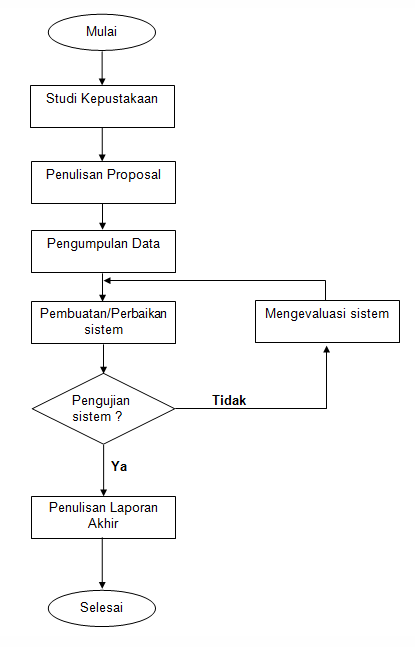
\includegraphics[width=0.7\textwidth]{gambar/1}  
 \caption{Tampilan Flowchart Pembuatan Proposal}
\end{figure}
\newpage
\section{Flowchart Pengembangan Sistem}
\begin{figure}[h]
\centering 
 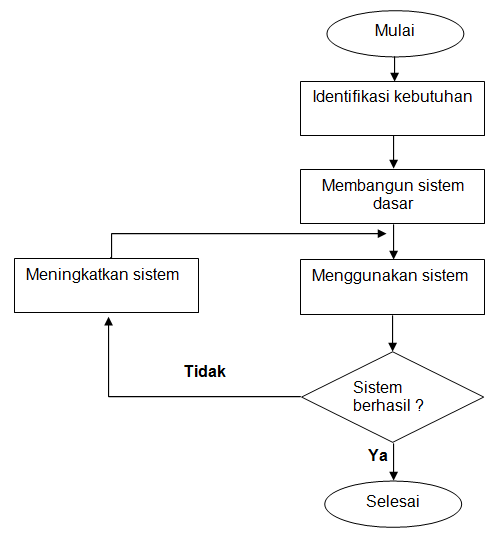
\includegraphics[width=1\textwidth]{gambar/2}  
 \caption{Tampilan Flowchart Pengembangan Sistem}
\end{figure}
\newpage
\section{Jadwal Kegiatan}
Penelitian direncanakan akan dilaksanakan selama empat bulan. Rincian rencana jadwal penelitian dicantumkan dalam tabel berikut.

\begin{center}
Tabel 3.1. Jadwal Penelitian.
\end{center}
\vspace{-0.5cm}
\begin{figure}[ht!]
  \centering
    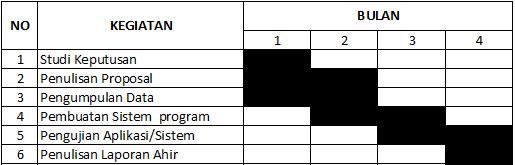
\includegraphics[width=13cm]{gambar/3}
\end{figure}

%-----------------------------------------------------------------
%Disini akhir masukan Bab
%-----------------------------------------------------------------

%-----------------------------------------------------------------
%Disini awal masukan untuk Daftar Pustaka
%-----------------------------------------------------------------
%%\nocite{Abel2010,Guerbas201350}
%%\bibliography{research-plan}
%%\bibliographystyle{plainnat}
\begin{thebibliography}{9}

\bibitem[satu(2013)]{satu01}
Budi Raharjo, Imam Heryanto, Arif Haryono, Mudah Belajar JAVA. Bandung : Informatika
\bibitem[dua(2013)]{dua02}
Supardi, Yanuar, Ir. 2007. Pemrograman Database dengan Java dan MySQL, Jakarta : PT.Gramedia.
\bibitem[tiga(2013)]{tiga03}
Hariyanto, Bambang, Ir, MT. 2003, Esensi-esensi Bahasa Pemrograman Java. Bandung : Informatika
\bibitem[empat(2013)]{empat04}
Dokumen online, www.wikipedia.com/sistem-informasi-manajemen.html, Sistem Informasi Manajemen, diakses pada Januari 2014

\bibitem[lima(2013)]{lima05}
Dokumen online, www.sharingilmujava.com/sistem-manajemen-keseretariatan-oraganisasi.html, Sistem, diakses pada Desember 2014

\end{thebibliography}
\addcontentsline{toc}{chapter}{DAFTAR PUSTAKA}
%-----------------------------------------------------------------
%Disini akhir masukan Daftar Pustaka
%-----------------------------------------------------------------

\end{document}